\epigraph{\textit{Logic is the foundation of the certainty of all the Knowledge we acquire.}}{-- \textup{Leonhard Euler}}

The main goal of this thesis is to create a tool capable of creating subsets out of a Knowledge graph. In this chapter, we will explore the possibility of implementing the Pregel framework in Rust, as well as a novel approach to the problem of Knowledge graph validation.

\section{Pregel-rs}

\subsection{Design}

\begin{figure}[ht]
    \centering
    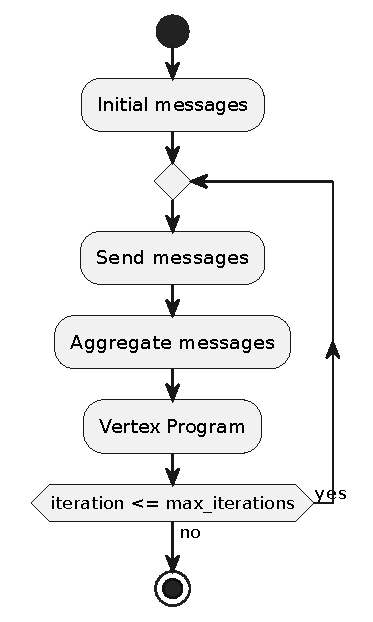
\includegraphics[width=0.33\textwidth]{diagrams/11-1_pregel.pdf}
    \caption{The Pregel framework as implemented in \texttt{pregel-rs}}
\end{figure}

\subsubsection{The Builder pattern}

\subsection{Implementation}

\section{PSchema-rs}

\subsection{The algorithm in a nutshell}

In this section, we will describe the algorithm that we are using to validate the Knowledge graph. The idea is to transform the given set of rules, \texttt{Shape} \texttt{Expression}, into a tree that is going to be traversed by the Pregel model that we have just described, namely, the subgraph matching algorithm. This idea takes inspiration from the \textit{Distributed subgraph matching algorithm} presented in \cite{Xu2019}; however, several modifications are introduced due to the requirements of our project.

\subsubsection{The \texttt{Shape} \texttt{Expression} tree}

Given a \texttt{Shape} \texttt{Expression} schema $\mathcal{S}$, we assume that it is a collection of labeled \texttt{Shape} \texttt{Expressions} that describe an RDF graph in terms of two main syntactic components\footnote{\url{https://shex.io/shex-primer/}}: \texttt{Triple Constraints}, \texttt{Shape References} and \texttt{Groupings of Triple Constraints}. The former is a triple pattern that describes a predicate-subject statement matched by the sub-setting algorithm. The second is another triple constraint where the subject is a reference to a \texttt{Shape}. The latter is a grouping of several of those constraints. The \texttt{Shape} \texttt{Expression} schema is going to be transformed into a tree, called \texttt{Shape} \texttt{Expression} tree, that is going to be traversed by the validation algorithm. This tree is going to be built recursively, and it is going to be traversed in a bottom-up fashion. This means that we are going to start by validating the leaves and then we are going to build the internal nodes, that is, the tree is going to be traversed in a \textit{reverse level order} fashion, as we need the children validated first for us to validate their parents. This is going to be done by an \texttt{iterator} that we will describe later on.

Putting this all together, \texttt{Shape} \texttt{Expressions} can be divided into two main categories according to the tree that they are going to generate, namely, \texttt{unary} and \texttt{n-ary} components. The former is going to generate a tree with a single node labeled with the identifier of the \texttt{Triple Constraint}, or, a single node with a single child in the case of a \texttt{Shape Reference}. The latter is going to generate a tree with a single node labeled with the identifier of the \texttt{Shape} that wraps the \texttt{Grouping} and with $n$ children. For each of the children, we are going to build their corresponding \texttt{Shape} \texttt{Expression} tree. This is going to be done recursively. For more information, see the \texttt{Shape} \texttt{Expression} tree definition.

\begin{definition}
    The \texttt{Shape} \texttt{Expression} tree $T$ is defined as follows. Having $\mathcal{S}$ a \texttt{Shape}, two main cases are possible:

    \begin{itemize}
        \itemsep0.5em
        \item If $\mathcal{S}$ is a \textit{unary} component, two cases are possible:
              \begin{itemize}
                  \itemsep0.25em
                  \item If $\mathcal{S}$ is a \texttt{Triple} \texttt{Constraint}, then $\mathcal{T}$ is a tree with a single node labeled with the identifier of the \texttt{Shape}.
                  \item If $\mathcal{S}$ is a \texttt{Shape Reference}, then $\mathcal{T}$ is a tree with a single node labeled with the identifier of the $\mathcal{S}$ shape and with a single child, $\mathcal{T}_1$, which is the \texttt{Shape} \texttt{Expression} tree of $\mathcal{S}_1$.
              \end{itemize}
        \item If $\mathcal{S}$ is a \textit{n-ary} component, one case is possible:
              \begin{itemize}
                  \itemsep0.25em
                  \item If $\mathcal{S}$ wraps a group of \texttt{Shapes}, then $\mathcal{T}$ is a tree with a single node labeled with the identifier of the $\mathcal{S}$ shape and with $n$ children,$\{\mathcal{T}_1, \mathcal{T}_2, ..., \mathcal{T}_n\}$, which are the \texttt{Shape} \texttt{Expression} trees of $\{\mathcal{S}_1, \mathcal{S}_2, ..., \mathcal{S}_n\}$, respectively.
              \end{itemize}
    \end{itemize}

    Note that the \texttt{Shape} \texttt{Expression} tree is going to be built recursively. Hence, the base case is the first item of this definition, and the recursive cases are the other two. In this manner, by chaining recursive cases, we can build a tree with an arbitrary depth.
\end{definition}

\begin{example}
    Following the definition of the \texttt{Shape} \texttt{Expression} tree, we are going to build the tree of the \texttt{Shape} \texttt{Expression} presented in example \ref{code:shex}.
    \vskip 0.5em
    \begin{minipage}{0.45\textwidth}
        \inputminted{shexc}{code/listings/6-4_shex.shex}
    \end{minipage}
    \begin{minipage}{0.45\textwidth}

    \end{minipage}
\end{example}

Note that nothing is said about the order of the children of the nodes. This is because the order of the children does not matter for the validation of the Knowledge graph. This is because the \texttt{Shape} \texttt{Expression} is a set of rules, and the order of the rules does not matter. Hence, the order of the children of the nodes does not matter either.

\subsubsection{The \texttt{Shape} \texttt{Expression} tree traversal}

The tree is going to be traversed in a bottom-up fashion. This means that we are going to start by validating the leaves and then we are going to build the internal nodes, that is, the tree is going to be traversed in a \textit{reverse level order} fashion. The reason for this is that we want to validate the leaves first because they are the ones that are going to be used for validating their parents. This is going to be done by an \texttt{iterator} that we will describe later on.

\subsubsection{The sub-graph matching algorithm}

The sub-graph matching algorithm that is going to be used for validating the Knowledge graph will traverse the Knowledge graph in a Pregel fashion and check whether the current node matches the \texttt{Shape} that is being validated. This is going to be done by the \texttt{iterator} that we have just described. According to this, it can be seen that several procedures should be considered; that is, we must properly define the following characteristics of the Pregel algorithm:

\begin{itemize}
    \itemsep0.5em
    \item The maximum number of iterations we want the algorithm to perform. If possible, we should establish an upper limit for the validation algorithm to iterate. As each superstep will possibly be a resource-heavy task, the lower the number of iterations, the better.
    \item At the beginning of the algorithm's execution an initial message is sent to all the nodes in the graph. After that, the first superstep is triggered.
    \item Both the message and the direction they follow are required to be defined. That is, we should establish a mechanism for nodes to know whether their neighbors conform to a certain \texttt{Shape} or not.
    \item As nodes may have several neighbors, a function for aggregating the set of messages having the node as the destination is also required.
    \item Having all the messages received and properly aggregated, the node should update its state according to what it has just collected.
\end{itemize}

\begin{pseudocode}[The PSchema algorithm as implemented in Rust]
    \includestandalone{code/algorithms/11-1_pschema}
\end{pseudocode}

\begin{theorem}
    Given a \texttt{Shape} \texttt{Expression} tree $\mathcal{T}$ and a Knowledge graph $\mathcal{G}$, let $h$ denote the height of $\mathcal{T}$; then if $h = 1$ the Pregel algorithm, denoted as $\mathcal{P}$, is going to validate the Knowledge graph $\mathcal{G}$ against $\mathcal{T}$ in $1$ superstep. If $h > 1$, then $\mathcal{P}$ is going to validate $\mathcal{G}$ against $\mathcal{T}$ in $h - 1$ supersteps. Formally, we can define the number of supersteps as follows:

    \begin{equation}
        \texttt{supersteps}(\mathcal{T}, \mathcal{G}) =
        \begin{cases}
            h     & \texttt{if } s = unary, \forall s \in \mathcal{T} \\
            h - 1 & \texttt{otherwise}
        \end{cases}
    \end{equation}
\end{theorem}

\begin{proof}
    Let us have $h$ the height of a \texttt{Shape} \texttt{Expression} tree $\mathcal{T}$, and let us denote $d_i$ the depth of the node $i$ in $\mathcal{T}$. Hence, at the superstep $h - d_i$, all the nodes at depth $d_i$ are going to be validated. As we traverse the tree in a \textit{reverse level order}, the previous definition holds. Hence, at the first superstep, the leaves are going to be validated, that is, at superstep 1, all the nodes at depth $h - 1$ are going to be validated. Then, at superstep 2, all the nodes at depth $h - 2$ are going to be validated; this is, at superstep $i$ nodes at depth $h - i$ are going to be validated. Thus, the tree is going to be traversed in $h$ supersteps. As the root is validated at the superstep $h - 0 = h$; note that the depth of the root node is 0, then, it can be seen that the tree is going to be traversed in $h$ supersteps.
\end{proof}

\subsection{Design}

\subsubsection{The \texttt{Iterator}}

\subsubsection{The \texttt{Validate} \texttt{trait}}

\subsubsection{Designing the \texttt{Shape} \texttt{Expressions}}

\paragraph{The \texttt{Shape} \texttt{Expression} \texttt{Composite}}

\paragraph{The \texttt{Shape} \texttt{Expression} \texttt{Adapter}}

\subsection{Optimizations}

\subsubsection{Parallelization}

The first optimization that we are going to consider is parallelization. The idea is to split the DuckDB dump into several chunks and then parse each of the chunks in parallel. This is going to be done by the first component of the tool. For this purpose, we are using \texttt{rayon}\footnote{\url{https://github.com/rayon-rs/rayon}}. This library is a data-parallelism API for Rust that provides several parallel iterators. Hence, we are using one to traverse the database in parallel. This can be done because each of the lines of the chunks of the dump is independent of each other. Thus, we can parse each of the entities in parallel without having to worry about synchronization issues. What's more, the \texttt{rayon} library is going to take care of the load balancing for us. This means that we do not have to worry about splitting the DuckDB dump into chunks of equal size. Lastly, \texttt{rayon} is also in charge of handling the thread pool for us and caring about the data-races that might arise.

What I like the most about \texttt{rayon} is the ease of transforming a sequential iterator into a parallel one. Let's have a look at an example of how this can be done:

\begin{minted}{rust}
    let lines = BufReader::new(file).lines();
    let lines = lines.into_par_iter();
\end{minted}

Whereas the first line creates a sequential iterator, the second one transforms it into a parallel one. This is done by calling the \texttt{into\_par\_iter} method on the iterator. Even if we have just shown a simple example, the actual solution is not far from what we have just shown above. See the code in the repository\footnote{\url{https://github.com/angelip2303/pschema-rs/blob/main/src/backends/duckdb.rs\#L64}} for a more detailed example:

\begin{code}[Parallel iterator over the DuckDB dump]
    \inputminted{rust}{code/listings/11-2_duckdb.rs}
\end{code}